\documentclass[11pt]{article}
\usepackage[margin=1.2in]{geometry}
\usepackage{graphicx}
\usepackage{fancyhdr}
\usepackage{nopageno}%removes number on titlepage
\usepackage[parfill]{parskip}
%\usepackage{subfig}
\usepackage{multirow}
\usepackage{caption}
\usepackage{subcaption}

\begin{document}
%% Cover page %%
\author{
\textbf{Chelsey Legacy} \\
Graduate Assistant \\
\texttt{calegacy@iastate.edu}
\and
\textbf{Lindong Zhou} \\
Graduate Assistant \\
\texttt{lindongz@iastate.edu}
\and
\textbf{Evan ``Pete" Walsh} \\
Graduate Assistant \\
\texttt{epwalsh@iastate.edu}
}
\title{
\textbf{Analysis of the Yelp Academic Dataset}\\
Factors that Affect the Ratings of Restaurants, Bars, Hotels, and Shopping Centers}
\date{
{\LARGE Iowa State University} \\
Department of Statistics \\
December 4, 2014}
\maketitle

\begin{abstract}
For this project we examined a Yelp Academic Data set with information pertaining to 250 of the closest businesses to 30 large universities. For our analysis we firs cleaned the dataset to get it into usable form. We then focused on analysis on restaurants, bars, hotels and shopping. By splitting the dataset into these smaller subsets we were able to find relationships between the variables and do a different analysis for each subset. For restaurants we find interesting relationships among reservations, noise level, delivery, takeout, price, and number of stars the business receives. We also find that service is key to a restaurants success. For bars we find that there are some relationships between the attributes of a bar will determine what type of group will venture to that bar. We also find that most bars serve American food, though other food are well represented. For hotels and shopping we find that it may not always mean better quality when paying more for services. And that people's reviews are not much affected by whether the place has a parking lot nearby or free wifi. Through this dataset we gain insight the relationships among many variables pertaining to a variety of sources.
\end{abstract}

%% End cover page %%

\newpage

\tableofcontents

\newpage

\pagenumbering{arabic}%starts numbering at "1"
\pagestyle{fancy}
\fancyhead[L]{Iowa State University}
\rhead{\thepage}
\rfoot{\today}
\cfoot{}%removes default page number at bottom center


\section{Introduction}

The Yelp Academic Dataset\footnote{$https://www.yelp.com/academic\_dataset$} provides data enthusiants with the exciting opportunity to explore an incredible collection of information regarding the characteristics and quality of hundreds of businesses across the United States, Canada, and the UK. This paper provides some thorough insight into the data using a variety of visualization techniques. 

....

This paper will procede as follows: Section 2 discusses the raw data and the steps that were taken to ``clean" the data into a more useful form. Section 3 examines the subset of data associated with restaurants, while sections 4, 5, and 6 examine the subsets associated with bars, hotels, and shopping, respectively. We conclude in section 7 by summarizing what we have found and offering several ideas for future studies.


\section{Data}


The Yelp Academic Dataset includes details and reviews on 250 of the closest businesses to 30 large universities, including the Arizona State, UNLV, the University of Edinburgh, the University of Wisconsin, and the University of Waterloo, to name a few. The raw data is in json format and contains five different types of json objects: \textbf{Business}, \textbf{Review}, \textbf{User}, \textbf{Check-in}, and \textbf{Tip}.

Each \textbf{Review} object represents an individual user-based review of a particular business. The unique encrypted business ID is given along with the date of the review, the number of stars (out of 5) that were awarded, the number and type of votes that the review received, and an optional text description provided by the user. \textbf{User} objects are unique to every person that has an active Yelp account. Each user has a name, a unique encrypted user ID, the number of votes they have cast, the average number of stars they have given, and the date they signed up for Yelp, among other things. A \textbf{Check-in} object represents the count and time of all the registered check-ins for a particular business, and \textbf{Tip} objects represent a tip given by user for a particular business. Tips include the user's ID, the business's ID, the date, and the message that the user gave. While these objects all provide a rich source of information, for the scope of this paper we will only be examing the \textbf{Business} objects.

\textbf{Business} objects are unique to business ID's, and include the following information:
\begin{itemize}
	\item the name of the business,
	\item the name of neighborhood in which the business is located,
	\item the city in which the business is located,
	\item the full address of the business,
	\item the exact latidude and longitude coordinates of the business,
	\item the average number of stars awarded to the business,
	\item the number of reviews received by the business,
	\item whether or not the business is still open,
	\item the hours that the business is open,
	\item the categories that the business falls under,
	\item and a number of different attributes which mostly concern restaurants and bars, such as whether or not smoking is allowed and the price range of the food.
\end{itemize}

To work with the data, we converted the set of all \textbf{Business} objects to a csv file in which the columns are variable names representing each aspect of a \textbf{Business} object, and each row corresponds to a unique business. Each different type of attribute was converted to its own character, numerical, or logical variable depending on what was appropriate. For example, the attribute \textbf{smoking} was converted to a logical variable where the value is ``true" if the smoking is allowed at the establishment, and ``false" if it is not allowed, while the attribute \textbf{price range} was converted to a numerical variable which ranges from 1 to 4.


\section{Restaurants}

Most of the data about restaurants in the Yelp Academic Dataset are concentrated around the following cities:
\begin{itemize}
	\item Madison, WI, 
	\item Las Vegas, NV,
	\item Pheonix, AZ,
	\item Waterloo, Ontario, Canada,
	\item and Edinburgh, Scotland.
\end{itemize}
Although the choice of cities is limited, the wealth of information coming from each city is abundant. All together, our data consists of 14,303 restaurants with 45 variables describing their attributes and the collective user sentiment towards each establishment. There is a significant number of restaurants in just about any subcategory that one can imagine. For example, Figure~\ref{fig:food01a} shows all of the restaurants classified as either ``hipster" or ``divey" near Pheonix, AZ that have televisions, offer live music, and have more than 35 reviews on Yelp. Figure~\ref{fig:food01b} shows all of the Asian and Indian food restaurants near Las Vegas, NV that offer take-out and have a full bar.

\begin{figure}[h]
\caption{Restaurant subsets near Pheonix, AZ and Las Vegas, NV.\label{fig:food01}}
\centering
\begin{subfigure}{0.45\linewidth}
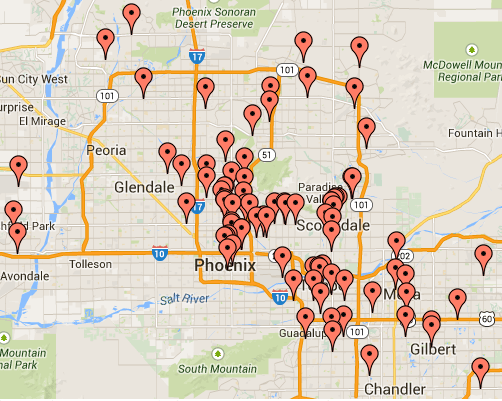
\includegraphics[width=\linewidth]{Figures/food_AZ.png}
\caption{\footnotesize{All restaurants near Pheonix, AZ classified as ``hipster" or ``divey" that have live music, TV's, and more than 35 reviews on Yelp.}}
\label{fig:food01a}
\end{subfigure}
\begin{subfigure}{0.45\linewidth}
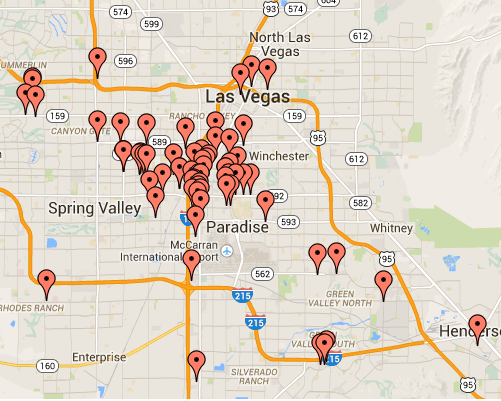
\includegraphics[width=\linewidth]{Figures/food_NV.png}
\caption{\footnotesize{All Asian and Indian food restaurants near Las Vegas, NV that offer take-out and have a full bar.}}
\label{fig:food01b}
\end{subfigure}
\end{figure}

\subsection{The Cost of Reservations}

One question we have explored with the data is whether restaurants that take reservations are more expensive and of higher quality than those that do not. Not suprisingly, it appears that one has to pay a premium, on average, to eat out at a restaurant that accepts reservations. Figure~\ref{fig:food_res_price} shows the average price level of restaurants by type that do or do not accept reservations. For each category, the price level is higher on average for restaurants that accept reservations.

There are a couple potential explanations for this. For one, it could just be that fancier restaurants feel they need to accept reservations to attract their target demographic. Perhaps people who are willing to spend a large amount on a meal will only do so if they know they will be seated right when they arrive. Or maybe restaurants that take reservations lose some money in transition time when open tables are kept unoccupied until the party that made the reservation arrives. The higher average price of restaurants that take reservations could just be making up for this inefficiency.

\begin{figure}[h]
\caption{Price scale of restaurants by type and whether they accept reservations.}
\centering
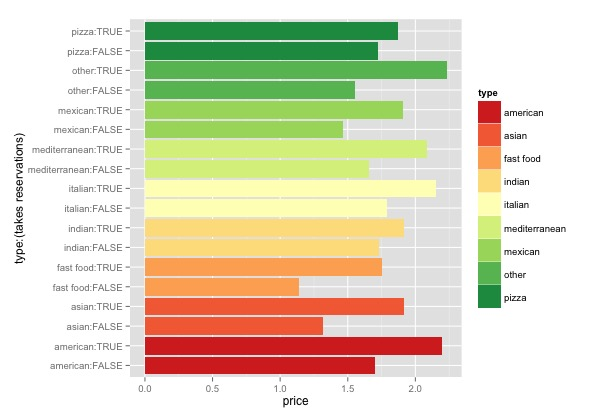
\includegraphics[width=0.7\linewidth]{Figures/food_res_price.jpeg}
\label{fig:food_res_price}
\end{figure}

Although a premium is payed to eat at restaurants that accept reservations, we find that the quality of the experience does not necessarily increase, as measured by the average stars awarded by Yelp users. Figure~\ref{fig:food_res_stars} compares the average stars received by each category by whether or not reservations are accepted. While the average number of stars is slightly higher for pizza, fast food, Asian, American, and ``other" style restaurants that take reservations, the average star count is actually lower for Mexican, Mediterranean, Italian, and Indian style restaurants.

\begin{figure}[h]
\caption{Rating of restaurants by type and whether they accept reservations.}
\centering
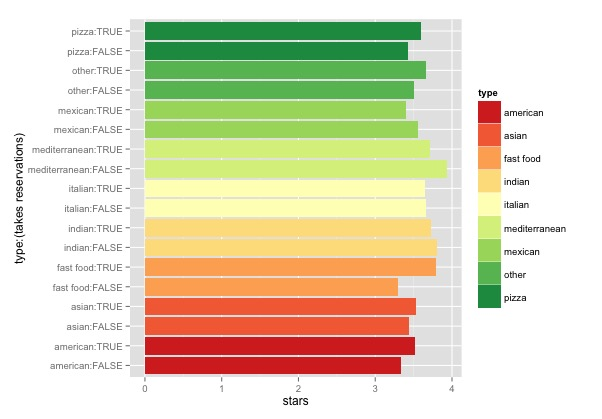
\includegraphics[width=0.7\linewidth]{Figures/food_res_stars.jpeg}
\label{fig:food_res_stars}
\end{figure}

The reason for this discrepancy is unclear. Maybe popular restaurants in certain categories just don't accept reservation because it would be too inefficient, and customers are fine with that. Price may also have something to do with it. Figure~\ref{fig:food_res_3} shows the rating of restaurants by type, whether they accept reservations, and price level. For Mexican restaurants, the average rating of low priced establishments is indistinguishable between those that accept reservations and those that do not. Yet for those in the third price level, the rating is clearly higher for those that do not take reservations. The same is true for Asian style restaurants while the opposite holds for Italian and American style restaurants. This could be because people who generally like to eat at pricier Italian and American food restaurants prefer to be able to make reservations, so these restaurants that allow reservations end up with higher ratings.

\begin{figure}[p]
\caption{Rating of restaurants by type, whether they accept reservations, and price level.}
\centering
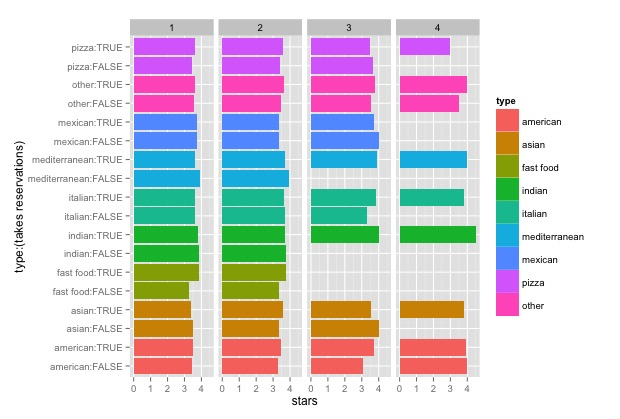
\includegraphics[width=0.8\linewidth]{Figures/food_res_3.jpeg}
\label{fig:food_res_3}
\end{figure}

\subsection{Loud can be Good, but not too Loud}

Another question we sought to answer was how noise pollution affects the quality of a dining experience, especially when we consider whether or not the establishment offers live music. One can imagine that people deliberately going out to eat at a restaurant with a band playing might bear a higher noise level, and thus not be as quick to penalize the restaurant for being too noisy in their review. We find that the data is consistent with this hypothesis.

For restaurants that offer live music, as shown in Figure~\ref{fig:food_noise}, loud places have a higher average rating than places with an average noise level. Yet very loud places have the lowest average rating. For restaurants that do not offer live music, the average rating decreases with the noise level.

\begin{figure}[p]
\caption{Rating of restaurants by their noise level and whether they host live music. The plot on the left shows the rating of restaurants by noise level that do not have live music, and the plot on the right shows the rating for restaurants with live music.}
\centering
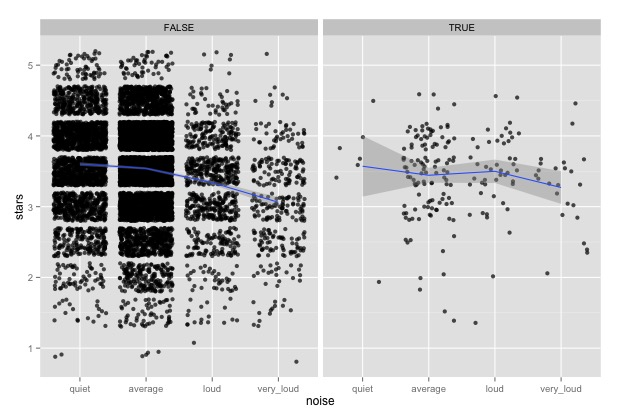
\includegraphics[width=0.7\linewidth]{Figures/food_noise.jpeg}
\label{fig:food_noise}
\end{figure}


\subsection{It's All About Service}

It will come as no surprise that service is a vital part of the service industry. Friendly, competent staff can make or break the dining experience. To illustrate the validity of this statement, we examined the \textbf{Tips} objects to see which words came up the most when Yelp users were describing either a really bad or really good restaurant experience. We first matched every single restaurant tip with the corresponding restaurant, and then sorted the tips by the average number of stars that each restaurant has. We then used a simple visualization technique on each set, called a wordcloud. 

A wordcloud is formed by displaying the most frequently occuring words from a set together in a random, or partly random, arrangement. The size of each word is weighted by how many times it appears in the set. A coloring scheme is often added to complement the size weighting.

We first took a random sample of 600 tips corresponding to restaurants with at least 4.5 stars, and 600 corresponding to restaurants with less than 2 stars. We then created a wordcloud for each set of tips after removing certain words like ``great," ``awesome," and ``love" from the high rating group and words like ``bad," ``terrible," and ``don't" from the low rating group, because those words are obvious and appeared so frequently that they ``clouded" out more interesting words. There were also other words like ``try," ``place," and ``get" that were removed from both groups for the same reasons. The resulting wordclouds are shown in Figures~\ref{fig:wordcloud_a}, for the high rating group, and~\ref{fig:wordcloud_b} for the low rating group.

\begin{figure}[h]
\caption{Wordclouds of tips for great restaurants and terrible restaurants.\label{fig:wordcloud}}
\centering
\begin{subfigure}{0.49\linewidth}
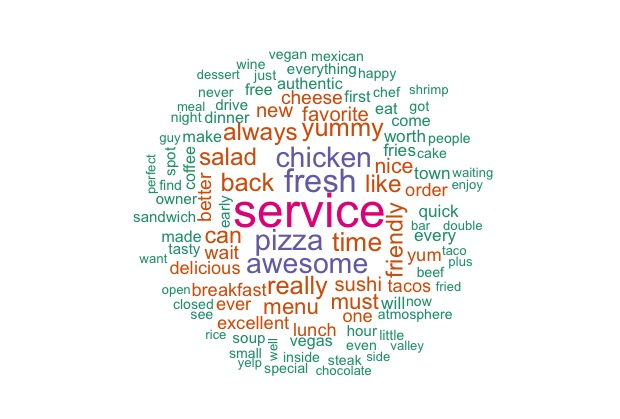
\includegraphics[width=\linewidth]{Figures/wordcloud_top.jpeg}
\caption{\footnotesize{Tips for restaurants with atleast 4.5 stars.}}
\label{fig:wordcloud_a}
\end{subfigure}
\begin{subfigure}{0.49\linewidth}
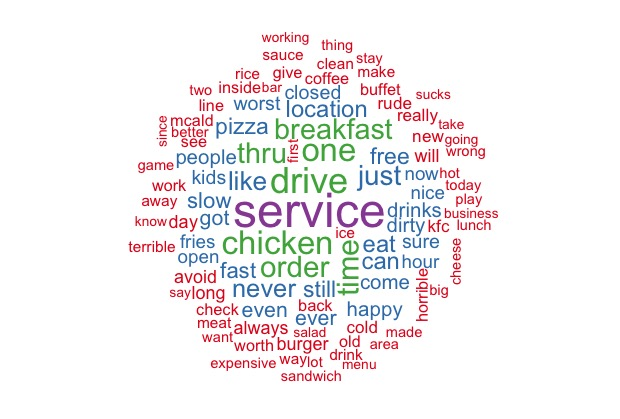
\includegraphics[width=\linewidth]{Figures/wordcloud_bottom.jpeg}
\caption{\footnotesize{Tips for restaurants with less than 2 stars.}}
\label{fig:wordcloud_b}
\end{subfigure}
\end{figure}

The interesting thing to notice here is that both wordclouds look extremely similar. Words like ``chicken," ``pizza," ``time," and ``order" are found in each set. Further, in both cases the word ``service" was the most frequent word. Thus, it seems that people with either really good or really bad experiences tend to comment on the same types of things, particularly when it comes to service.



\subsection{Delivery vs. Takeout}

\begin{figure}[h!]
  \caption{Plot of the counts of each type of food filled by if they have delivery or not.}
  \centering
  \label{delivery}
    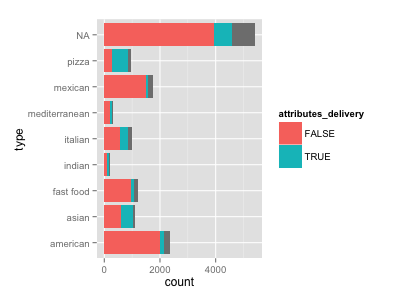
\includegraphics[width=0.75\textwidth]{Figures/delivery.png}
\end{figure}
\begin{figure}[h!]
  \caption{Plot of if a restaurant does takeout orders colored by if they do deliveries and faceted by the type of food the restaurant serves.}
  \centering
  \label{takeout}
    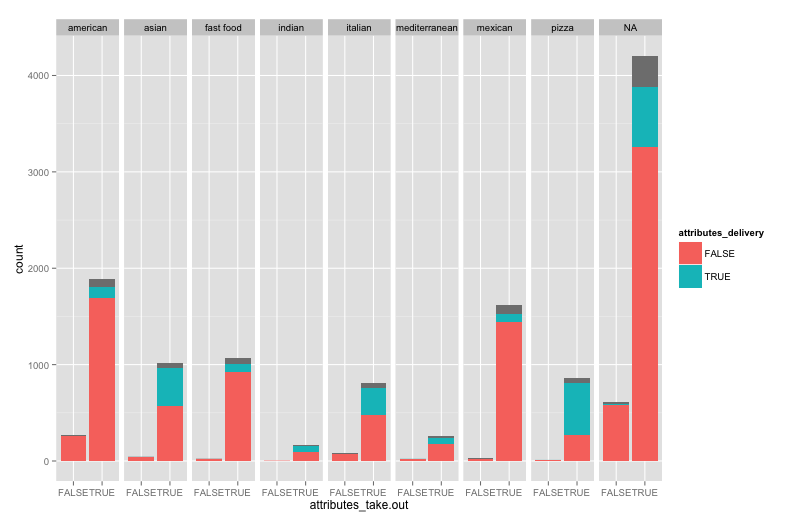
\includegraphics[width=0.9\textwidth]{Figures/takeoutdelivery.png}
\end{figure}
Now we know have gained some insight into restaurants' price and reservation style, but what about when you do not want to go eat at the restaurant? Some days there is little time for cooking, so people commonly call out for delivery or take out.  But what types of food are most likely to have delivery or takeout?  In other words, if we are ordering out, what is it likely we will be able to have delivered to us and what can we pick up on our way home? In 
Figure~\ref{delivery} we can see that the food types that most likely have delivery are those that serve pizza, Asian, or possibly Italian.  Most likely you will not be able to find an American or fast food place that delivers.  This could be due to the fact that some of these food do not stay good if they sit too long.  Food like pizza and rice are fine to sit for a while,  are easy to keep warm and fresh tasting, and can also be easily reheated. Thus, these are qualities that make them good options for delivery.  However, American food, or fast food like burgers and fries are not good if they sit too long, and do not reheat to the quality they were when they left the restaurant.  Thus, there are fewer, if any of these places that offer delivery.

We can see in more detail in Figure~\ref{takeout} that restaurants of all types are much more likely to offer takeout than delivery to customers.  We can also see that the restaurant is more likely to offer delivery if they offer a takeout option.  Restaurants of all types may be more inclined to offer delivery than takeout for a number of reasons.  They could only have a limited number of people working and do not want to spare any or pay extra people to deliver the food.  Delivery also means transportation costs for the business, and as discussed above it means more time for the food to decrease in quality while a driver makes several deliveries.  However, takeout is a great option for restaurants, because they get to sell more food, without have to seat as many people in the restaurant.  Takeout also reduces the responsibility of the quality of the food once it arrives at its destination.  If it took the customer a long time to get home and the food is not as good as it once was, this is not the restaurant's fault.  



\section{Bars}

The Business dataset contains a lot of information that can be used to analyze the relationship between different aspects of bar culture.  In order to analyze the bars available in the dataset, the data was subset to get rid of any businesses that did not have a full bar.  Looking at only the businesses with a full bar gives us insight into locations that serve from a full bar such as clubs, hotels, select restaurants, lounges, bowling alleys, and other various entertainment locations.  Through analyzing this data we can explore what types of food are servied at bars (if any), if lower ratings indicate a bar could shut down, and the type of activities that might take place at a given bar.

\subsection{Food}

\begin{figure}[h!]
  \caption{Plot of the number of stars a restaurant received filled with the type of food served at the bar.}
  \centering
  \label{food}
    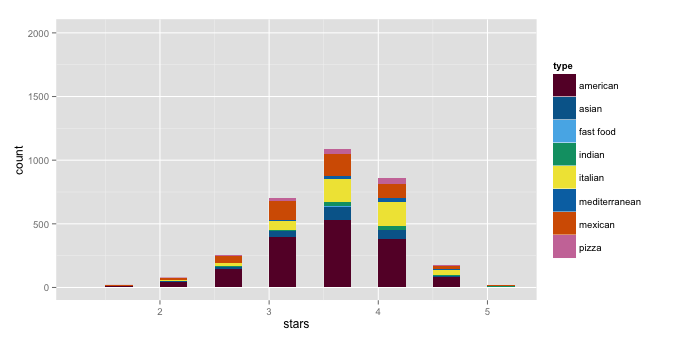
\includegraphics[width=0.75\textwidth]{Figures/Food_bars.png}
\end{figure}

Though not all bars serve food, many bars in restaurants do which begs the question; what is the most common food served in bars?  In order to investigate this question a qplot of the number of starts given to each bar filled with a count of the food types for each different rating will give us the information and more.  This data revealed, unsurprisingly, that the most common food served in American bars is American food (burgers, fries, etc). Through further analysis it is determined that 50$\%$ of the bars that serve food served primarily American style food.  We can see that the majority of each bar of star, no matter what the rating, is colored for American food.  However, looking more closely at the graph we can see that there is some unexpected information.  From Figure~\ref{food} we can see that there are a wide number of food options for people looking for full bars.  Along with American, Italian and Mexican are also abundant options making up 16$\%$ and 16.7$\%$ respectively.  Another piece of information we can infer from this graphic is that along with the plot of the stars a bar receives being a normal distribution, there also is a consistency in the number of each type of food being represented at each level of stars a bar receives.  Thus, we can see there is no preference for food when looking for a certain quality bar. A bar is equally likely to serve American food whether it receives 1 star or 5 stars.  This could be further investigated through hypothesis testing for difference in proportions.

\subsection{Stars}
\begin{figure}[h!]
  \caption{Plot of the number of stars a bar received colored by whether or not they are open or closed}
  \centering
  \label{open}
    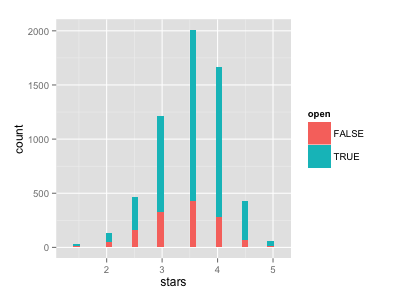
\includegraphics[width=0.75\textwidth]{Figures/barstatus.png}
\end{figure}
The purpose of yelp is to provide review of businesses for others in the community to take into consideration.  Since this dataset provides the number stars a bar receives and the status of the bar (open or closed) as of when the data was collected.  I decided to investigate the idea that possibly if the bar has lower ratings it has more of a chance of being closed.  It is hard to discern any sort of relationship from the plot, except that there are more restaurants open than closed.  However, if inspected closely looking at the extreme endpoints of the graph you can see it appears the percent of open restaurants at the 5 star level is higher than the percent of 1 star restaurants that are open. In order to look into this further I created several subsets of the data.  I created a subset of data for 2 stars(1 star had 0 observations), 3.5 stars (which is the median of the data), and 5 stars.  I then found the percent of open bars for each level.  I found that the 2 stars had 64.3$\%$ open, the 3.5 stars had 78.4$\%$ and 5 stars had 82.1$\%$ open.  As we can see the percentages of bars open increases as the number of stars the bar is rated increases.  Though we can make no assumptions of causation, this is still an interesting trend tp consider for further more complex analysis.

\subsection{Popular Features}
\begin{figure}
\centering
\begin{subfigure}{.5\textwidth}
  \centering
  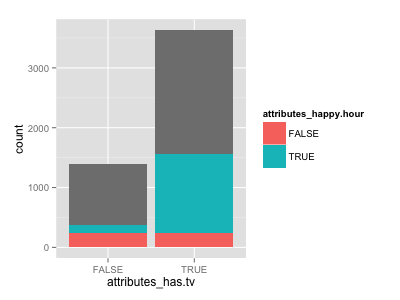
\includegraphics[width=1\linewidth]{Figures/tvhappyhour.png}
  \caption{Plot indicating whether or not the bar as a tv, colored by if it has happy hour specials}
  \label{happy}
\end{subfigure}%
\begin{subfigure}{.5\textwidth}
  \centering
  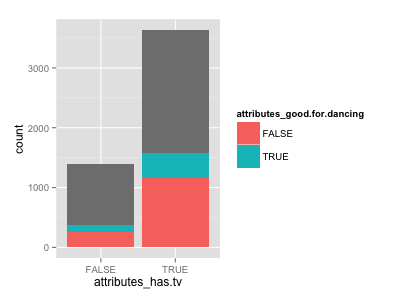
\includegraphics[width=1\linewidth]{Figures/tvdancing.png}
  \caption{Plot indicating whether or not the bar as a tv, colored by if it is good for dancing}
  \label{dance}
\end{subfigure}
\caption{}
\label{}
\end{figure}

\vspace{5mm}
Each bar in a community has its own unique features, special pricing promotions, or atmosphere.  Some bars are good for dancing, watching televisions broadcasting sports games, happy hour, or some are more quiet and laid back for just talking and relaxing with friends.  What are the relationships between these variables, if any?  I wanted to find characteristics for each of the  different atmospheres a bar may have: romantic, intimate, touristy, hipster, divey, classy, trendy, upscale, and casual.  However, it quickly became clear that there are not many bars in each of these categories.  Most bars are just classified as casual.  Thus, there wasn't much to investigate.



Next, I thought it would be interesting to look at features of bars with televisions.  Since, not all bars have televisions there must be certain characteristics for those that choose to have a television and those that do not.   In  Figure~\ref{happy} we can see that most bars that have a tv also have happy hour specials.  These are probably more causal places that people go after work to relax with coworkers and friends.  We can gain even more insight into the bars with tvs when we look at  Figure~\ref{dance}.  In this plot it is interestingly apparent that if a bar has a tv it is more likely that it is not good for dancing.  This again reinforces that the bars with televisions are more of a relaxed atmosphere to hang out and chat or watch sports.  Most likely a place like this would be an in inappropriate atmosphere for a group looking to go dancing.  Places people go dancing are more apt to be louder places people go later at night, when happy hour specials would be over and there would be no need for televisions while dancing.  






\section{Hotels}

We created a subset of the Yelp data to get only businesses whose categories contain “Hotels”. Focusing on the variables that have relatively few missing values, we included price range, wifi, location and rating in our analysis. Most of hotels in the dataset are located in the US states of Arizona, Nevada and Wisconsin as well as Edinburgh in Scotland. The dataset is helpful for us to find out whether popularity, price level, wifi and location influence the rating of a hotel.

Popularity does not necessarily mean better products and services. This statement is supported by Figure 12 which shows the distribution of ratings by popularity. We determined the popularity of a hotel based on the total number of user reviews. Hotels that have fewer than 100 reviews are considered as least popular, whereas hotels with more than 100 and 1000 reviews have medium and high popularity respectively. Across levels of popularity, there is no significant difference in the distribution of ratings. 4-star reviews are posted on the website most frequently, followed by 5-star and 3-star reviews. Thus, switching to a better promoted hotel does not seem to affect people’s lodging experience.

\begin{figure}[h!]
           \caption{Histogram of the relative frequency of ratings of hotels by popularity}
	\centering
	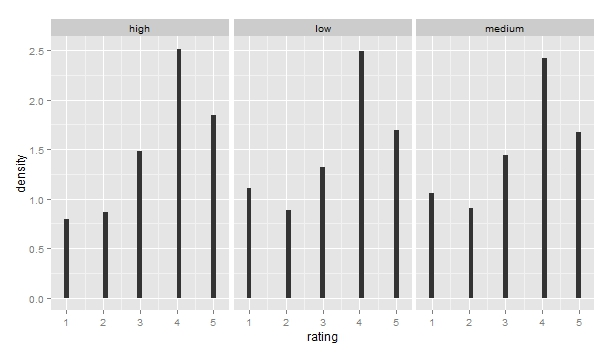
\includegraphics[width=0.5\textwidth]{Figures/hotels1.jpeg}
           \label{hotels1}
\end{figure}

Wifi does not seem to matter as well. Figure 13 shows the distribution of ratings by price range and availability of wifi. Within each price range, the distribution pattern appears roughly the same whether Wifi is free, paid or not provided. However, the graph suggests a correlation between price range and customer satisfaction. High-priced hotels receive better reviews compared to budget hotels. One possible explanation is that overnight stay in a hotel is mostly attractive to high-end customers who value quality of amenities and customer service more than just price. This observation supports the commonly held belief among travelers that you get what you pay for.

\begin{figure}[h!]
           \caption{Histogram of the relative frequency of ratings of hotels by price range and whether Wifi is free, paid or unavailable}
	\centering
	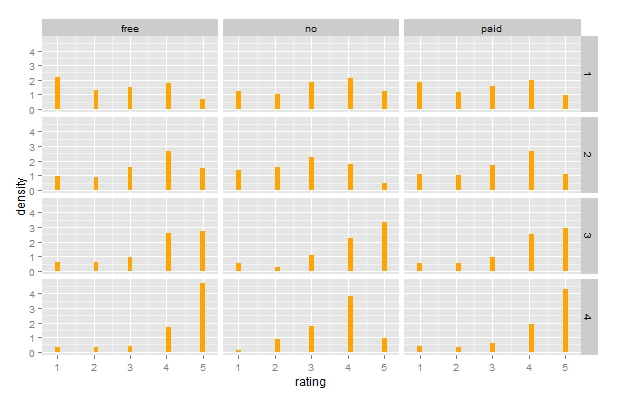
\includegraphics[width=0.5\textwidth]{Figures/hotels2.jpeg}
           \label{hotels2}
\end{figure}

Paying more for a better service might not be true outside the United States. The notion of “you get what you pay for” is clearly refuted by Figure 14 which shows the distribution of ratings by price range and region. While high-priced hotels are still rated higher than budget hotels in Arizona, Nevada and Wisconsin, the ratings of hotels in Edinburgh seem to be consistent across price levels. Perhaps European customers receive equal treatment regardless of how much they pay, whereas American customers have to pay more to get better treatment. Nevertheless, we cannot justify the claim without examining more data about American and European hotels.

\begin{figure}[h!]
           \caption{Histogram of the relative frequency of ratings of hotels by price range and region}
	\centering
	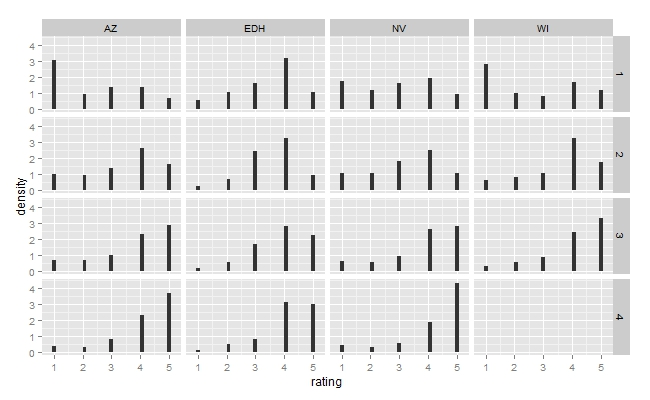
\includegraphics[width=0.5\textwidth]{Figures/hotels3.jpeg}
           \label{hotels3}
\end{figure}

\section{Shopping}

To examine all types of shops in the dataset, we subset the data to get only businesses whose categories contain “Shopping”. Considering missing values, we included variables price range, parking lot, location and rating in our analysis. Like hotels, most of the shops in the dataset are located in Arizona, Nevada, Wisconsin and Edinburgh. We use the data to explore the effects of popularity, price range, parking lot and location on the rating of a retail store.

Figure 15 again supports the statement that popularity is not associated with better products and services. We determined the popularity of a retail store using the same criteria (see Section 5). The graph shows that the pattern does not change much as popularity goes up. So, customers do not seem to improve their shopping experience by joining a crowd.

\begin{figure}[h!]
           \caption{Histogram of the relative frequency of ratings of shops by popularity}
	\centering
	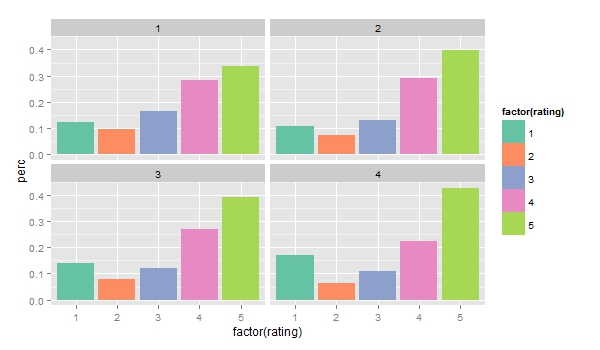
\includegraphics[width=0.5\textwidth]{Figures/shopping1.jpeg}
           \label{shopping1}
\end{figure}

Figure 16 shows the distribution of the ratings by price range and availability of parking. Whether or not there are parking lots nearby, the stores are rated roughly the same. It is interesting to see, however, that pricey stores receive more polarized reviews than low-cost stores. In the highest price range, we find more 5-star reviews and more 1-star reviews at the same time. Customers seem to either love or hate the stores that charge them very high prices. One might argue that retail customers are more diverse than hotel customers. In other words, average people tend to focus more on price than quality. Without looking at the demographics of customers, we never know if this argument is true.

\begin{figure}[h!]
           \caption{Histogram of the relative frequency of ratings of shops by price range and whether a parking lot is available or not}
	\centering
	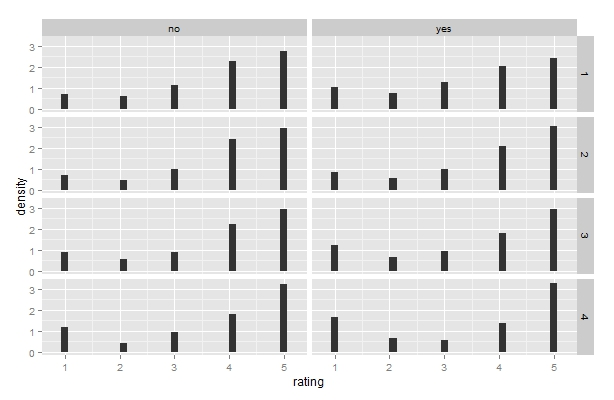
\includegraphics[width=0.5\textwidth]{Figures/shopping2.jpeg}
           \label{shopping2}
\end{figure}

Figure 17 shows another different trend in the distribution of ratings of retail stores in Edinburgh. While pricey stores still receive more polarized reviews than low-cost stores in three states, especially Arizona, the ratings of stores in Edinburgh are again consistent across price levels. Assuming that the demographics are the same everywhere, one could possibly say that quality is better reflected by price in European stores. This implies that the quality of an American product sometimes does not justify its price. Again, we cannot verify the statement without any more information.

\begin{figure}[h!]
           \caption{Histogram of the relative frequency of ratings of shops by price range and region}
	\centering
	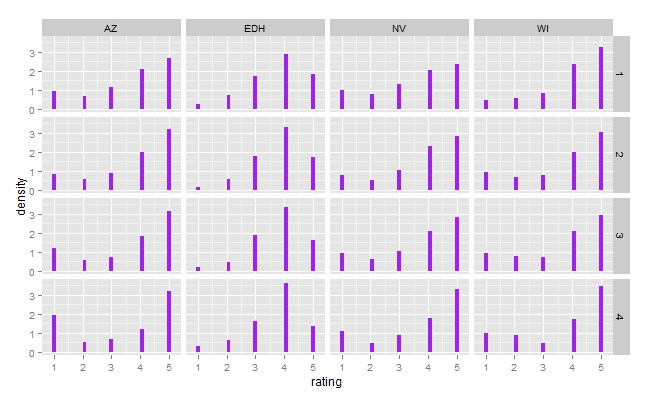
\includegraphics[width=0.5\textwidth]{Figures/shopping3.jpeg}
           \label{shopping3}
\end{figure}


\section{Conclusion}

The Yelp Academic Dataset has provided us information on a variety of businesses including restaurants, bars, hotels, and shops.  We have used the abundance of data to find key relationships between the available variables and their respective businesses.  For example, we have found that reservations, price, noise level, takeout, delivery, and foremost service are key variables that provide interesting relationships for restaurant data.  We have also found that features such as food type, if a restaurant has a tv, or if it is good for dancing all provide insight into what type of atmosphere we will find at a bar.  When evaluating  hotels and shopping we have found that popularity does not always reflect the quality of the service we will receive.  This data set has provided us with many insights into possible relationships between not only these variables, but also human culture and tendencies.  Though it is impossible to make solid conclusions about any of the relationships we have found based on our limited dataset, we have still come up with some interesting relationships and found even more questions about this topic that could be used for further research on the subject.



\end{document}